\documentclass[../../main.tex]{subfiles}
\begin{document}

\subsection*{10.7}
Due guide conduttrici parallele, distanti $b = 20\ cm$, sono chiuse ad un estermo da un resistore con $R =4\ \Omega$.\\
Lungo le guide può scivolare senza attrito, sotto l'azione del proprio peso, una sbarretta conduttrici di massa $m = 10^{-2}\ kg$.\\
Il dispositivo è immerso in un campo magnetico $B=1\ T$ uniforme e costante, ortogonale al piano del circuito.\\
Calcolare come variano nel tempo la velocità v(t) della sbarretta e la corrente i(t), i valori limite $v_\infty$ e $i_\infty$, l'energia $W_1$ dissipata nel circuito per ogni centimetro percorso dalla sbarretta in queste condizioni.\\
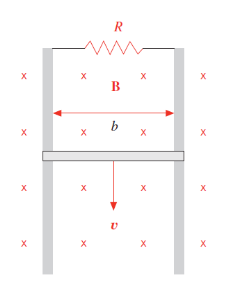
\includegraphics[scale=0.3]{e_10_7.png}
\subsubsection*{Formule utilizzate}
\subsubsection*{Soluzione punto a}
$\varepsilon_i = -\frac{d\Phi(\vec{B})}{dt}$\tab\tab$\varepsilon_i = vbB$\\
che tende a generare una corrente $ i = \frac{vbB}{R}$ in verso antiorario. Pertanto sulla barretta si esercita una forza verso l'alto pari a: $F_{mag} = \frac{vbB}{R}bB$ opposta alla forza mg.\\
Da $a = \frac{dv}{dt} = \frac{F}{m}$ segue che: $\frac{dv}{dt} = g- \frac{iBb}{m} = g-\frac{B^2b^2}{mR}v$\\
Separando le variabili e integrando si ha:\\
$\int_0^{v(t)}\frac{dv}{g-\frac{B^2b^2}{mR}v}=\int_0^tdt$\\
$-\frac{mR}{B^2b^2}\left[log\left(g-\frac{B^2b^2}{mR}v(t)\right)-log(g)\right] = t$\\
$log\left(1-\frac{B^2b^2}{mgR}v(t)\right) = -\frac{B^2b^2}{mR}t$\\
$\frac{B^2b^2}{mR} = 1\ s^{-1}$\\
$v(t) = \frac{mgR}{B^2b^2}\left(1-e^{\frac{-B^2b^2t}{mR}}\right) = 9.8 * \left(1-e^{\frac{-B^2b^2t}{mR}}\right)\ \frac{m}{s}$\\
Di conseguenza: $i(t) = \frac{Bb}{R}v(t) = \frac{mg}{Bb}\left(1-e^{\frac{-B^2b^2t}{mR}}\right)$\\
I valori limite sono:\\
$v_\infty = \frac{mgR}{B^2b^2} = 9.8\ \frac{m}{s}$\\
$i_\infty = \frac{mg}{Bb} = 0.49\ A$\\
In condizioni stazionarie l'energia dissipata per ogni spostamento $\Delta x = 1\ cm$ risulta quindi:\\
$W_1 = Ri^2_\infty\Delta t =Ri^2_\infty\frac{\Delta x}{v_\infty} = 9.8 * 10^{-4}\ J$\\
Uguale alla perdita di energia potenziale gravitazionale della sbarretta ($mg \Delta x$)
\subsubsection*{Soluzione punto b}
\newpage

\end{document}